%
% characteristics.tex -- XXX
%
% (c) 2019 Prof Dr Andreas Mueller
%
\section{Charakteristiken}
\rhead{Charakteristiken}
\subsection{Ein unlösbares Cauchy-Problem}
Wir untersuchen jetzt, unter welchen Voraussetzungen sich das Cauchy-Problem
für eine hyperbolische partielle Differentialgleichung eindeutig lösen lässt.
Um besser zu verstehen, was dabei schief gehen kann, betrachten wir die
hyperbolische partielle Differentialgleichung
\[
\partial_x\partial_y u=0,
\]
und geben die Anfangswerte die
\begin{align*}
u(0,y)&=u_0(y)
\\
\partial_xu(0,y)&=v_0(y)
\end{align*}
vor.
Aus der Differentialgleichung schliessen wir, dass $\partial_y u$
nicht von $x$ abhängt. Somit kann auch $u$ nicht von $x$ abhängen,
die Anfangsbedingung für $\partial_xu(0,y)$ ist also redundant,
sie kann nur erfüllt werden, wenn $v_0(y)=0$.
Die Lösung ist $u(x,y)=u_0(y)$.

Da aber auch $\partial_x\partial_yu=\partial_y\partial_xu$, ist auch
$u(x,y)=g(x)$ eine Lösung der Differentialgleichung. Da diese
Lösung nicht von $y$ abhängt, kann auch die Anfangsbedingung $u(0,y)=u_0(y)$
nicht erfüllt werden. Offenbar ist das Cauchy-Problem nicht lösbar, wenn die
Funktionswerte und Ableitungen auf der Geraden $x=0$ vorgegeben werden.
Ursache dafür ist, dass aus der Differentialgleichung nicht alle zweiten
Ableitungen bestimmt werden können. Die zweite partielle Ableitung
nach $\partial_x^2u(0,y)$ ist unbestimmt.

\subsection{Streifen}
Das Cauchy-Problem kann also nur dann lösbar sein, wenn die Funktionswerte
und die ersten partiellen Ableitungen entlang einer Kurve
auch alle zweiten Ableitungen eindeutig bestimmen.
Wir versuchen daher
diejenigen Kurven zu bestimmen, auf denen dies nicht möglich ist.
Wir gehen aus von der Differentialgleichung
\begin{equation}
a\frac{\partial^2 u}{\partial x^2}
+
2b\frac{\partial^2 u}{\partial x\partial y}
+
c\frac{\partial^2 u}{\partial y^2}
+
d\frac{\partial u}{\partial x}
+
e\frac{\partial u}{\partial y}
+
fu
=g,
\label{charequation}
\end{equation}
Da wir vor allem an den zweiten Ableitungen interessiert sind, bringen
wir alle anderen Terme auf die rechte Seite, und kürzen die neue
rechte Seite mit $h$ ab:
\begin{equation}
a\frac{\partial^2 u}{\partial x^2}
+
2b\frac{\partial^2 u}{\partial x\partial y}
+
c\frac{\partial^2 u}{\partial y^2}
=
g
-
d\frac{\partial u}{\partial x}
+
e\frac{\partial u}{\partial y}
+
fu
=h.
\notag
\end{equation}
Ausserdem betrachten wir eine Kurve
$t\mapsto(x(t),y(t))$.
Entlang der Kurve sind die Anfangswerte
und die partiellen Ableitungen
\begin{equation}
\left.
\begin{aligned}
u(x(t),y(t))&=u(t)\\
\frac{\partial u}{\partial x}(x(t),y(t)) &= p(t)\\
\frac{\partial u}{\partial y}(x(t),y(t)) &= q(t)
\end{aligned}
\qquad
\right\}
\label{charanfangs}
\end{equation}
vorgegeben. Diese Vorgaben nennt man einen {\em Streifen}
(Abbildung~\ref{skript:streifen}).

\begin{figure}
\centering
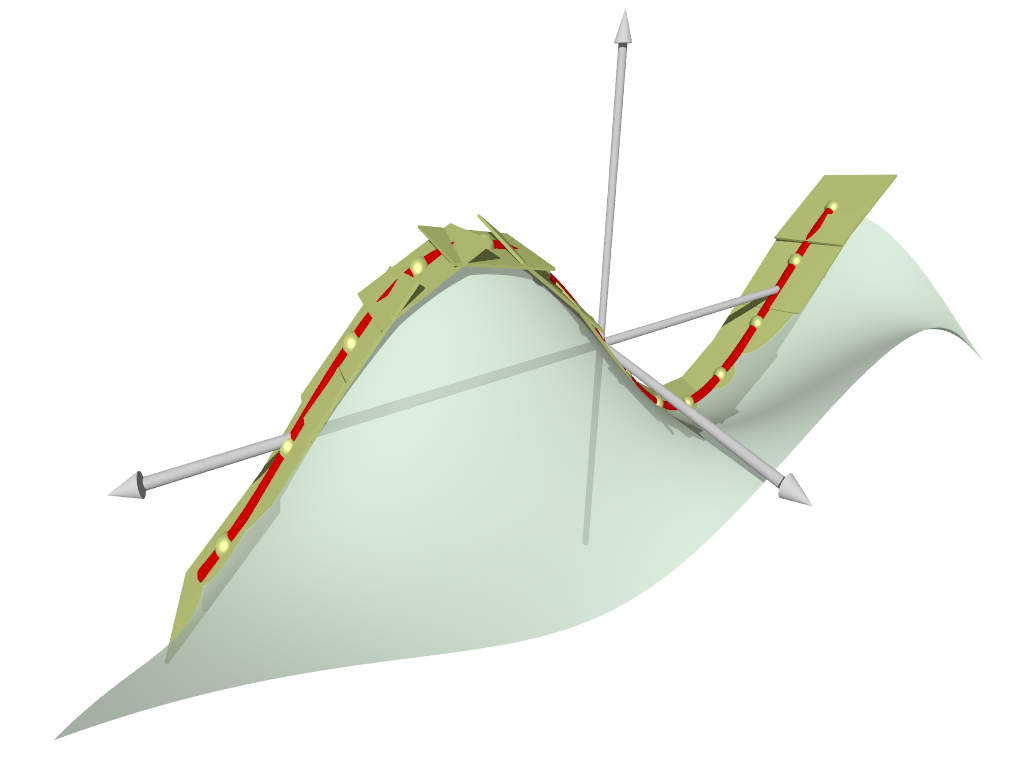
\includegraphics[width=\hsize]{../common/3d/streifen0.png}
\caption{Ein Streifen besteht aus der Vorgabe von Anfangskurve (rot)
und Tangentialbenen.
Die grüne Fläche ist Lösungsfläche der Wellengleichung mit 
dem Streifen als Anfangsbedingung.
\label{skript:streifen}}
\end{figure}

\begin{figure}
\centering
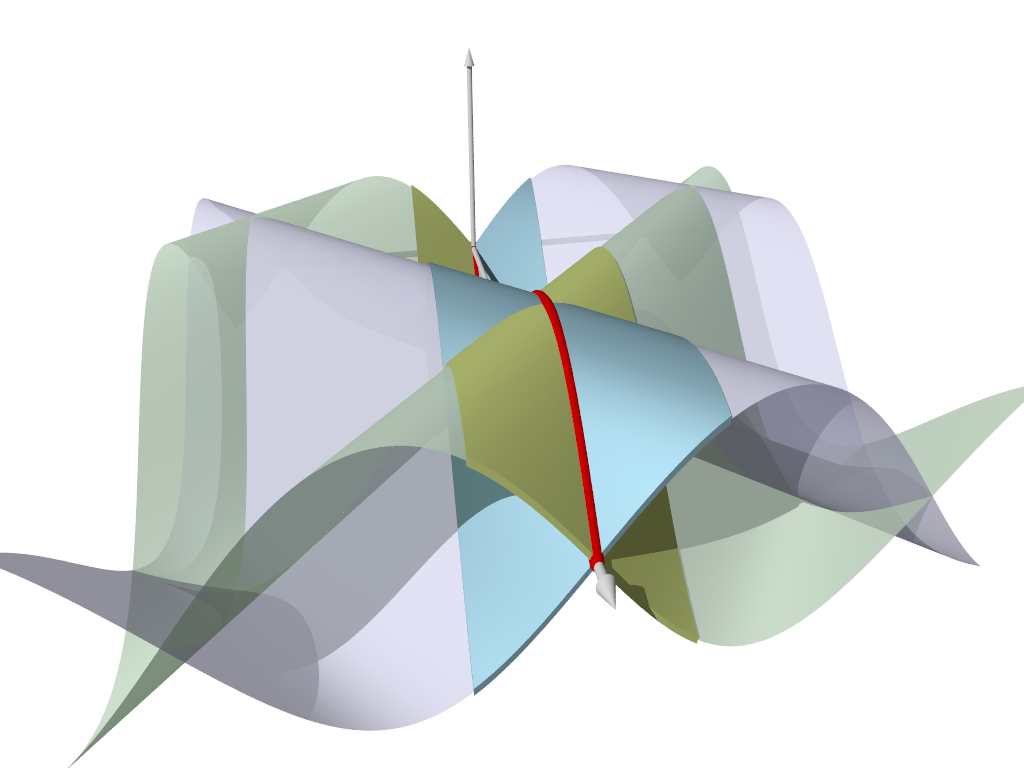
\includegraphics[width=\hsize]{../common/3d/streifen2.png}
\caption{Entlang der gemeinsamen roten Kurve haben die beiden
Lösungsflächen der Wellengleichung verschiedene Tangentialebenen,
also verschiedene Streifen. 
Der Streifen legt die Lösung eindeutig fest.
\label{skript:streifen:eindeutig}}
\end{figure}

\begin{figure}
\centering
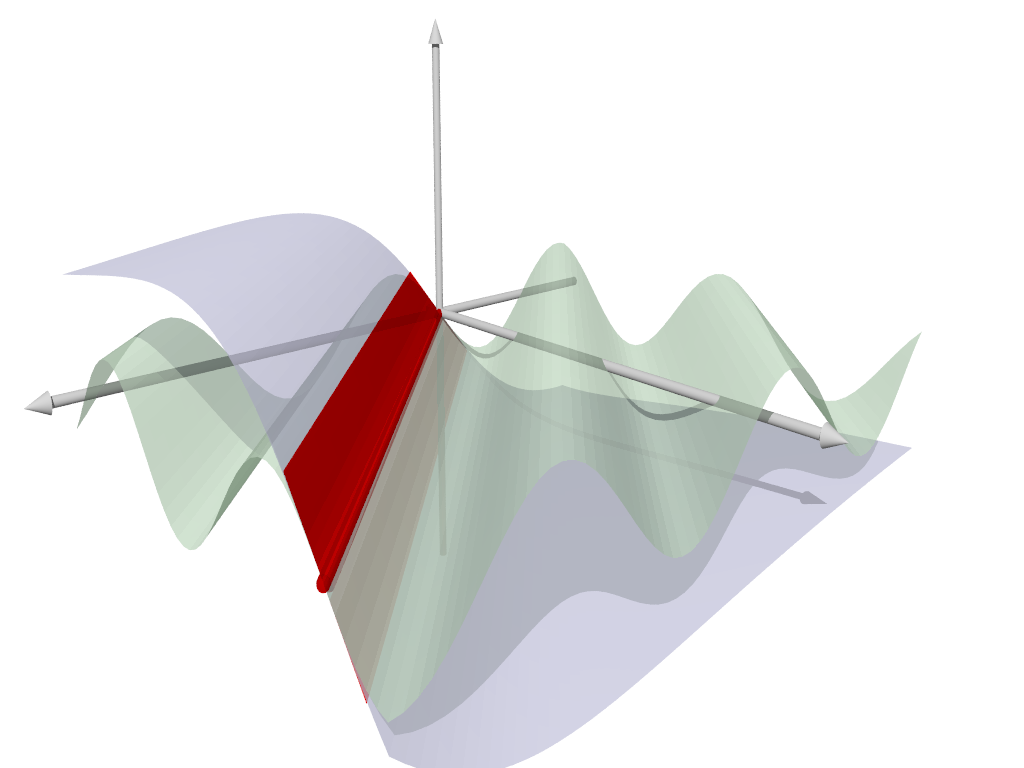
\includegraphics[width=\hsize]{../common/3d/streifen1.png}
\caption{Charakteristiken sind nicht geeignet als Anfangskurven,
weil ein Streifen entlang einer Charakteristik die Lösungsfläche
nicht eindeutig zu bestimmen braucht. Die Abbildung zeigt zwei Lösungen
der Wellengleichung, die sich in dem roten Streifen berühren.
\label{skript:streifen:zweideutig}}
\end{figure}

Die Funktionen $u(t)$, $p(t)$ und $q(t)$ sind nicht ganz willkürlich.
Leitet man nämlich die erste der Gleichungen (\ref{charanfangs}) nach
$t$ ab, findet man
\[
\dot{u}(t)=\frac{d}{dt}u(t)
=
\frac{d}{dt}u(x(t),y(t))
=
\frac{\partial u}{\partial x}(x(t), y(t))\frac{d}{dt}x(t)
+
\frac{\partial u}{\partial y}(x(t), y(t))\frac{d}{dt}y(t).
\]
Die partiellen Ableitungen sind aber ebenfalls in (\ref{charanfangs})
vorgegeben, es muss also die Beziehung
\begin{equation}
\dot{u}(t)= p(t)\dot{x}(t) + q(t)\dot{y}(t)
\label{cauchydatarestriction}
\end{equation}
gelten.

\subsection{Charakteristiken}
Die Vorgabe eines Streifens bestimmt die Lösung einer hyperbolischen
partiellen Differentialgleichung meistens eindeutig.
In Abbildung~\ref{skript:streifen:eindeutig} zeigt zwei verschiedene
Lösungen der Wellengleichung, die entlang der $t$-Achse zwar die
gleiche Anfangskurve, aber verschiedene Tangentialebenen und damit
verschiedene Streifen haben.

Leitet man die letzten zwei Gleichungen von (\ref{charanfangs}) nach $t$ ab,
erhält man
\[
\begin{linsys}{3}
\dot p(t)
&=&
\partial_x\partial_xu(x(t),y(t))\,\dot x(t)
&+&
\partial_x\partial_yu(x(t),y(t))\,\dot y(t)
& &
\\
\dot q(t)
&=&
& &
\partial_x\partial_yu(x(t),y(t))\,\dot x(t)
&+&
\partial_y\partial_yu(x(t),y(t))\,\dot y(t)
\end{linsys}
\]
Zusammen mit der Differentialgleichung haben wir also die folgenden
drei Gleichungen für die rot hervorgehobenen zweiten partiellen Ableitungen:
\[
\begin{linsys}{4}
a{\color{red}\displaystyle\frac{\partial^2 u}{\partial x^2}}
&+&
2b{\color{red}\displaystyle\frac{\partial^2 u}{\partial x\partial y}}
&+&
c{\color{red}\displaystyle\frac{\partial^2 u}{\partial y^2}}
&=&
h(t)
&=&
g-dp(t)-eq(t)-fu\\
\dot x(t)
{\color{red}\displaystyle\frac{\partial^2 u}{\partial x^2}}
&+&
\dot y(t)
{\color{red}\displaystyle\frac{\partial^2 u}{\partial x\partial y}}
& &
&=&
\dot p(t)
& &
\\
& &
\dot x(t)
{\color{red}\displaystyle\frac{\partial^2 u}{\partial x\partial y}}
&+&
\dot y(t)
{\color{red}\displaystyle\frac{\partial^2 u}{\partial y^2}}
&=&
\dot q(t)
& &
\end{linsys}
\]
Dieses lineare Gleichungssystem für die zweiten partiellen Ableitungen
hat die Koeffizientenmatrix
\[
\begin{pmatrix}
a&2b&c\\
\dot x(t)&\dot y(t)&0\\
0&\dot x(t)&\dot y(t)
\end{pmatrix}.
\]
Es ist genau dann nicht oder nicht eindeutig lösbar, wenn die Determinante
verschwindet
\begin{align*}
0&=\left|\begin{matrix}
a&2b&c\\
\dot x(t)&\dot y(t)&0\\
0&\dot x(t)&\dot y(t)
\end{matrix}\right|
\\
&=a\dot y(t)^2-2b\dot x(t)\dot y(t)+c\dot x(t)^2
\end{align*}

\begin{definition}
Die Charakterisitiken einer Differentialgleichung der Form (\ref{charequation})
sind die Kurven $t\mapsto(x(t),y(t))$, für die die Anfangswerte (\ref{charanfangs})
die zweiten partiellen Ableitungen nicht eindeutig bestimmen.
\end{definition}

\begin{satz}
\label{charakteristikendgl}
Die Charakteristiken einer partiellen Differentialgleichung (\ref{charequation})
erfüllen  die Differentialgleichung
\[
a\dot y(t)^2-2b\dot x(t)\dot y(t)+c\dot x(t)^2=0.
\]
\end{satz}

\subsection{Charakteristische Streifen}
Wir wählen jetzt eine Charakteristik $t\mapsto(x(t),y(t))$.
Uns interessiert nur der Fall, in dem es unendlich viele
Lösungen für die zweiten Ableitungen gibt. Dieser tritt dann
ein, wenn auch die Determinanten
\[
\left|
\begin{matrix}
h&2b&c\\
\dot p(t)&\dot y(t)&0\\
\dot q(t)&\dot x(t)&\dot y(t)
\end{matrix}
\right|
,
\quad
\left|
\begin{matrix}
a&h&c\\
\dot x(t)&\dot p(t)&0\\
0&\dot q(t)&\dot y(t)
\end{matrix}
\right|
,
\quad
\left|
\begin{matrix}
a&2b&h\\
\dot x(t)&\dot y(t)&\dot p(t)\\
0&\dot x(t)&\dot q(t)
\end{matrix}
\right|
\]
verschwinden, wobei $h=g-dp(t)-eq(t)-fu(x(t),y(t))$.
Es genügt dabei, eine einzige Determinante zu wählen,
wir wählen die zweite:
\begin{align*}
a\dot p(t)\dot y(t)-h\dot x(t)\dot y(t)+c\dot x(t)\dot q(t)&=0
\end{align*}
Zusammen mit der Bedingung~(\ref{cauchydatarestriction})
%\[
%\dot u=p(t)\dot x(t)+q(t)\dot y(t)
%\]
haben wir jetzt drei Gleichungen, welche die Grössen 
$x$, $y$, $u$, $p$ und $q$ erfüllen müssen, damit die zweiten
Ableitungen auf unendlich viele Arten bestimmt sind.

\begin{definition}
Ein Streifen entlang einer Charakteristik, der zusätzlich die
Bedingung 
\[
a\dot p(t)\dot y(t)-h\dot x(t)\dot y(t)+c\dot x(t)\dot q(t)=0
\]
erfüllt, heisst ein {\em charakteristischer Streifen}.
\end{definition}

Es ist also möglich, dass sich Integralflächen einer Differentialgleichung
in einer Kurve schneiden, dort sogar berühren, aber trotzdem verschieden
sind. Notwendigerweise bilden die Tangentialebenen
entlang der Schnittkurve einen charakteristischen Streifen.

\begin{satz}
\label{skript:satz:charakteristiken}
Berühren sich zwei verschiedene Integralflächen entlang einer
Kurve, dann stellen diese Kurve zusammen mit den zugehörigen Tangentialebenen
einen charakteristischen Streifen dar.
\end{satz}

Abbildung~\ref{skript:streifen:zweideutig} zeigt zwei Lösungen der
Wellengleichung, die sich entlang einer Charakteristik berühren.
Nach Satz~\ref{skript:satz:charakteristiken} ist der rote Streifen ein
charakteritischer Streifen.

\begin{proof}[Beweis]
Offenbar gibt es mindestens zwei Lösungen der Differentialgleichung
durch die gegebene Kurve, die ausserdem die gleichen Tangentialebenen
haben. Die Kurve und die Tangentialebenen bestimmen die Lösung nicht
eindeutig, sie bilden also einen charakteristischen Streifen.
\end{proof}

\subsection{Beispiele}
\subsubsection{Wellengleichung}
Die Charakteristiken der Wellengleichung
\begin{equation}
\partial_t^2u-a^2\partial_x^2u=0
\label{hyperbolisch:wellengleichung}
\end{equation}
sind Kurven $s\mapsto(t(s),x(s))$, die die Gleichung
\begin{align*}
\left(
\frac{dx(s)}{ds}\right)^2-a^2\left(\frac{dt(s)}{ds}\right)^2&=0
\\
\frac{dx(s)}{ds}
&=
\pm a\frac{dt(s)}{ds}
\\
\Rightarrow
\frac{dx}{dt}=\pm a
\end{align*}
erfüllen. Dies sind Geraden mit der Steigung $\pm a$.
\begin{figure}
\begin{center}
\includegraphics[width=0.8\hsize]{../common/images/char-2.pdf}
\end{center}
\caption{Charakteristiken der
Wellengleichung~(\ref{hyperbolisch:wellengleichung})
\label{hyp:wellen}}
\end{figure}
Abbildung~\ref{hyp:wellen} zeigt die Charakteristiken.

\subsubsection{Die Gleichung $\partial_x\partial_yu=0$} Die Bedingung für die
Charakteristiken lautet in diesem Fall
\[
-\dot x(t)\dot y(t)=0
\]
Eine der Ableitungen muss also verschwinden, was nur für Kurven
möglich ist, die parallel zur $x$- oder $y$-Achse verlaufen.
Die Abbildung \ref{hyp:dxdy} zeigt die Charakteristiken.
\begin{figure}
\begin{center}
\includegraphics[width=0.8\hsize]{../common/images/char-3.pdf}
\end{center}
\caption{Charakteristiken der hyperbolischen
partiellen Differentialgleichung
$\partial_x\partial_yu=0$.
\label{hyp:dxdy}}
\end{figure}

\subsubsection{Gekrümmte Charakteristiken}
Die partielle Differentialgleichung
\begin{equation}
\partial_t^2u-x^2\partial_x^2u=0
\label{hyperbolisch:gekruemmt}
\end{equation}
ist für $x\ne 0$ hyperbolisch.
Ihre Charakteristiken erfüllen die Gleichung
\begin{align*}
x'(s)^2-x^2t'(s)^2&=0
\\
xt'&=\pm  x'
\\
\frac{d}{ds}t&=\pm\frac{d}{ds}\log x
\\
t&=\pm\log x+C
\\
x&=x_0e^{\pm t}
\end{align*}
Die Charakteristiken sind also Exponentialkurven. In Abbildung \ref{hyp:exp}
sind die Charakteristiken für das positive Zeichen rot eingezeichnet, die
Charakteristiken für das negative Zeichen dagegen grün.
\begin{figure}
\begin{center}
\includegraphics[width=0.8\hsize]{../common/images/hypexp-1.pdf}
\end{center}
\caption{Charakteristiken der für $x\ne 0$ hyperbolischen
partiellen Differentialgleichung~(\ref{hyperbolisch:gekruemmt}).
\label{hyp:exp}}
\end{figure}

Diese Gleichung beschreibt die Wellenausbreitung in einem Medium,
in dem die Wellengeschwindigkeit mit grösser werdendem $x$ ebenfalls
zunimmt. Die Exponentialkurven deuten an, wie die Wellenbewegung nach ``aussen''
immer schneller wird.

\subsection{Charakteristiken für elliptische und parabolische PDGL}
Die oben entwickelte Theorie der Charakteristiken kann selbstverständlich
auch auf elliptische und hyperbolische PDGL angewendet werden.
Im elliptischen Fall hat die Differentialgleichung der Charakteristiken
\[
a\dot y(t)^2-2b\dot x(t)\dot y(t)+c\dot x(t)^2=0
\]
gar keine Lösung, da der Ausdruck nur dann verschwindet, wenn $\dot x(t)=0$
und $\dot y(t)=0$.

Für parabolische PDGL wird der Ausdruck bei Wahl eines geeigneten
Koordinatensystems zu
\[
-\kappa t'(s)^2=0
\]
dies ist nur möglich, wenn $t$ konstant ist. Die Charakteristiken
sind in diesem Falle also Geraden parallel zur $x$-Achse.
Tatsächlich ist es mit der Differentialgleichung und
den Anfangsbedingungen alleine nicht
möglich, die zweite Ableitung nach $t$ entlang einer solchen Geraden
zu bestimmen.

\subsection{Einige interessante Sätze}

\begin{satz}Jede Integralfläche kann mit einer Schar
charakteristischer Streifen bedeckt werden.
\end{satz}

\begin{proof}[Beweis]
Sei $u$ eine Lösung der Differentialgleichung, die die Integralfläche beschreibt.
Die Differentialgleichung von Satz \ref{charakteristikendgl}
beschreibt in jedem Punkt des Definitionsbereichs zwei Kurven $t\mapsto(x(t),y(t))$,
offenbar kann man den Definitionsbereich mit einer Schar solcher Kurven
überdecken.
Setzen wir diese Kurven in $u(x,y)$, $\partial_xu(x,y)$
und $\partial_yu(x,y)$ ein, erhalten wir eine Schar von charakteristischen
Streifen.
\end{proof}

\begin{satz}Überdeckt eine Schar charakteristischer Streifen
eine Fläche $S$, gegeben durch eine Funktion $u(x,y)$, und hat
diese Funktion stetige Ableitungen bis zur zweiten Ordnung,
dann ist $u$ eine Lösung der Differentialgleichung.
\end{satz}

\begin{proof}[Beweis]
Die charakteristischen Streifen erfüllen die Gleichungen
\begin{equation}
\begin{gathered}
a\dot y(t)^2-2b\dot x(t)\dot y(t)+c\dot x(t)^2=0,
\\
a\dot p(t)\dot y(t)-h\dot x(t)\dot y(t)+c\dot x(t)\dot q(t)=0,
\\
\dot u(t)=p(t)\dot x(t)+q(t)\dot y(t).
\end{gathered}
\label{alle}
\end{equation}
Nennen wir die zweiten Ableitungen von $u$ entlang einer Charakteristik
\begin{align*}
R&=\partial_x^2u(x(t),y(t)),
\\
S&=\partial_x\partial_yu(x(t),y(t)),
\\
T&=\partial_y^2u(x(t),y(t)),
\end{align*}
können wir schreiben
\begin{align*}
\dot p(t)&=R(t)\dot x(t)+S(t)\dot y(t)\qquad\text{und}\\
\dot q(t)&=S(t)\dot x(t)+T(t)\dot y(t)
\end{align*}
Setzen wir dies in die zweite Gleichung von (\ref{alle}) ein, erhalten wir
\begin{align*}
a(R\dot x+S\dot y)\dot y-h\dot x\dot y+c\dot x(S\dot x+T\dot y)&=0
\\
\Rightarrow \qquad(aR-h+cT)\dot x\dot y+aS\dot y^2 +cS \dot x^2&=0.
\end{align*}
Multiplizieren wir die erste Gleichung von (\ref{alle}) mit $S$ und subtrahieren
sie, erhalten wir
\[
(aR+2bS+cT-h)\dot x\dot y=0.
\]
Ausgeschrieben ist der Klammerfaktor
\[
a\partial_x^2u+2b\partial_x\partial_yu+c\partial_y^2u-h=0
\]
Also die ursprüngliche Differentialgleichung.
\end{proof}
Dieser Satz besagt, dass man die hyperbolische Differentialgleichung dadurch
lösen kann, dass man charakteristische Streifen sucht. Dazu genügt
es aber, ein System von gewöhnlichen Differentialgleichungen
für die Funktion $x$, $y$, $p$, $q$, $R$, $S$ und $T$
zu lösen.

